\documentclass[1p]{elsarticle_modified}
%\bibliographystyle{elsarticle-num}

%\usepackage[colorlinks]{hyperref}
%\usepackage{abbrmath_seonhwa} %\Abb, \Ascr, \Acal ,\Abf, \Afrak
\usepackage{amsfonts}
\usepackage{amssymb}
\usepackage{amsmath}
\usepackage{amsthm}
\usepackage{scalefnt}
\usepackage{amsbsy}
\usepackage{kotex}
\usepackage{caption}
\usepackage{subfig}
\usepackage{color}
\usepackage{graphicx}
\usepackage{xcolor} %% white, black, red, green, blue, cyan, magenta, yellow
\usepackage{float}
\usepackage{setspace}
\usepackage{hyperref}

\usepackage{tikz}
\usetikzlibrary{arrows}

\usepackage{multirow}
\usepackage{array} % fixed length table
\usepackage{hhline}

%%%%%%%%%%%%%%%%%%%%%
\makeatletter
\renewcommand*\env@matrix[1][\arraystretch]{%
	\edef\arraystretch{#1}%
	\hskip -\arraycolsep
	\let\@ifnextchar\new@ifnextchar
	\array{*\c@MaxMatrixCols c}}
\makeatother %https://tex.stackexchange.com/questions/14071/how-can-i-increase-the-line-spacing-in-a-matrix
%%%%%%%%%%%%%%%

\usepackage[normalem]{ulem}

\newcommand{\msout}[1]{\ifmmode\text{\sout{\ensuremath{#1}}}\else\sout{#1}\fi}
%SOURCE: \msout is \stkout macro in https://tex.stackexchange.com/questions/20609/strikeout-in-math-mode

\newcommand{\cancel}[1]{
	\ifmmode
	{\color{red}\msout{#1}}
	\else
	{\color{red}\sout{#1}}
	\fi
}

\newcommand{\add}[1]{
	{\color{blue}\uwave{#1}}
}

\newcommand{\replace}[2]{
	\ifmmode
	{\color{red}\msout{#1}}{\color{blue}\uwave{#2}}
	\else
	{\color{red}\sout{#1}}{\color{blue}\uwave{#2}}
	\fi
}

\newcommand{\Sol}{\mathcal{S}} %segment
\newcommand{\D}{D} %diagram
\newcommand{\A}{\mathcal{A}} %arc


%%%%%%%%%%%%%%%%%%%%%%%%%%%%%5 test

\def\sl{\operatorname{\textup{SL}}(2,\Cbb)}
\def\psl{\operatorname{\textup{PSL}}(2,\Cbb)}
\def\quan{\mkern 1mu \triangleright \mkern 1mu}

\theoremstyle{definition}
\newtheorem{thm}{Theorem}[section]
\newtheorem{prop}[thm]{Proposition}
\newtheorem{lem}[thm]{Lemma}
\newtheorem{ques}[thm]{Question}
\newtheorem{cor}[thm]{Corollary}
\newtheorem{defn}[thm]{Definition}
\newtheorem{exam}[thm]{Example}
\newtheorem{rmk}[thm]{Remark}
\newtheorem{alg}[thm]{Algorithm}

\newcommand{\I}{\sqrt{-1}}
\begin{document}

%\begin{frontmatter}
%
%\title{Boundary parabolic representations of knots up to 8 crossings}
%
%%% Group authors per affiliation:
%\author{Yunhi Cho} 
%\address{Department of Mathematics, University of Seoul, Seoul, Korea}
%\ead{yhcho@uos.ac.kr}
%
%
%\author{Seonhwa Kim} %\fnref{s_kim}}
%\address{Center for Geometry and Physics, Institute for Basic Science, Pohang, 37673, Korea}
%\ead{ryeona17@ibs.re.kr}
%
%\author{Hyuk Kim}
%\address{Department of Mathematical Sciences, Seoul National University, Seoul 08826, Korea}
%\ead{hyukkim@snu.ac.kr}
%
%\author{Seokbeom Yoon}
%\address{Department of Mathematical Sciences, Seoul National University, Seoul, 08826,  Korea}
%\ead{sbyoon15@snu.ac.kr}
%
%\begin{abstract}
%We find all boundary parabolic representation of knots up to 8 crossings.
%
%\end{abstract}
%\begin{keyword}
%    \MSC[2010] 57M25 
%\end{keyword}
%
%\end{frontmatter}

%\linenumbers
%\tableofcontents
%
\newcommand\colored[1]{\textcolor{white}{\rule[-0.35ex]{0.8em}{1.4ex}}\kern-0.8em\color{red} #1}%
%\newcommand\colored[1]{\textcolor{white}{ #1}\kern-2.17ex	\textcolor{white}{ #1}\kern-1.81ex	\textcolor{white}{ #1}\kern-2.15ex\color{red}#1	}

{\Large $\underline{12a_{0425}~(K12a_{0425})}$}

\setlength{\tabcolsep}{10pt}
\renewcommand{\arraystretch}{1.6}
\vspace{1cm}\begin{tabular}{m{100pt}>{\centering\arraybackslash}m{274pt}}
\multirow{5}{120pt}{
	\centering
	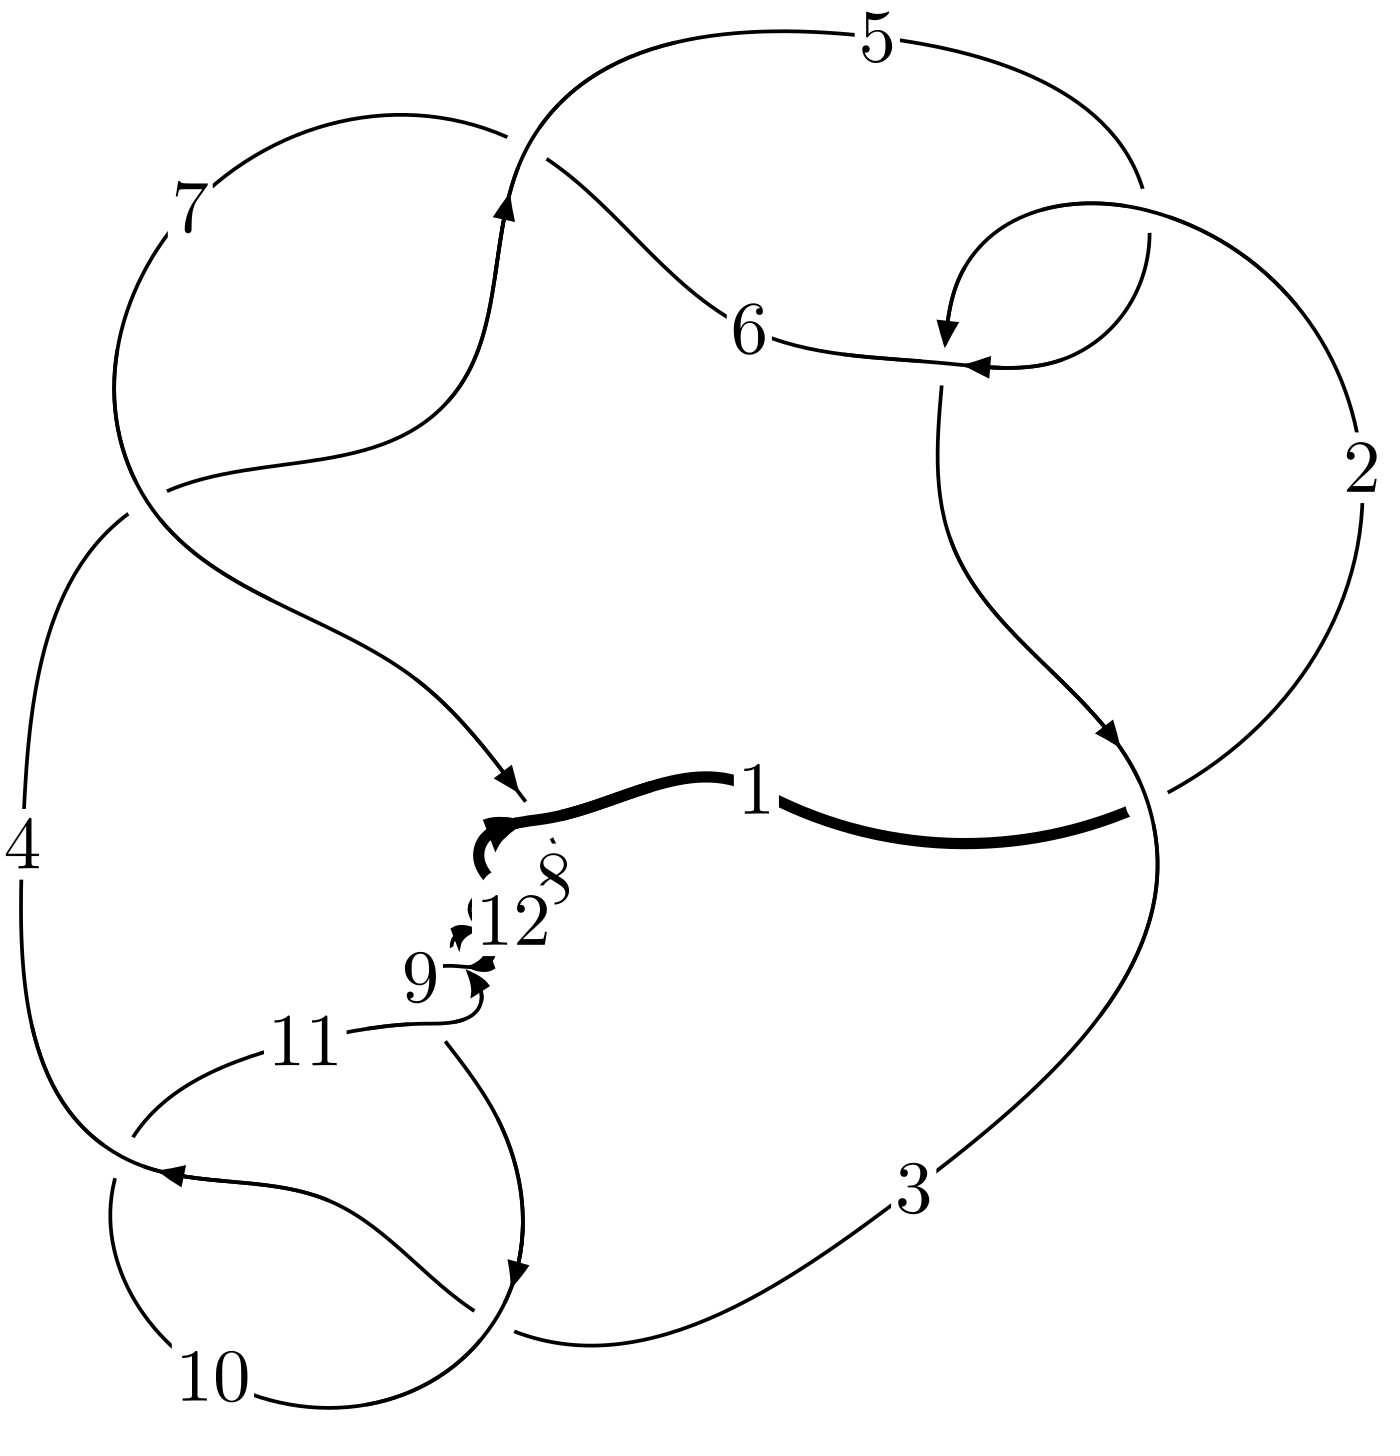
\includegraphics[width=112pt]{../../../GIT/diagram.site/Diagrams/png/1226_12a_0425.png}\\
\ \ \ A knot diagram\footnotemark}&
\allowdisplaybreaks
\textbf{Linearized knot diagam} \\
\cline{2-2}
 &
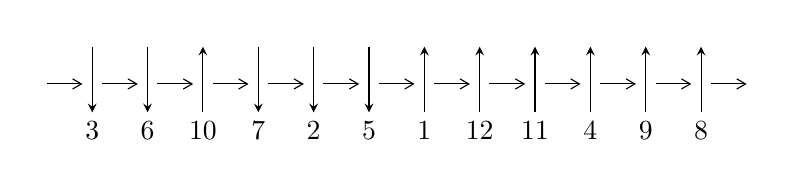
\begin{tikzpicture}[x=20pt, y=17pt]
	% nodes
	\node (C0) at (0, 0) {};
	\node (C1) at (1, 0) {};
	\node (C1U) at (1, +1) {};
	\node (C1D) at (1, -1) {3};

	\node (C2) at (2, 0) {};
	\node (C2U) at (2, +1) {};
	\node (C2D) at (2, -1) {6};

	\node (C3) at (3, 0) {};
	\node (C3U) at (3, +1) {};
	\node (C3D) at (3, -1) {10};

	\node (C4) at (4, 0) {};
	\node (C4U) at (4, +1) {};
	\node (C4D) at (4, -1) {7};

	\node (C5) at (5, 0) {};
	\node (C5U) at (5, +1) {};
	\node (C5D) at (5, -1) {2};

	\node (C6) at (6, 0) {};
	\node (C6U) at (6, +1) {};
	\node (C6D) at (6, -1) {5};

	\node (C7) at (7, 0) {};
	\node (C7U) at (7, +1) {};
	\node (C7D) at (7, -1) {1};

	\node (C8) at (8, 0) {};
	\node (C8U) at (8, +1) {};
	\node (C8D) at (8, -1) {12};

	\node (C9) at (9, 0) {};
	\node (C9U) at (9, +1) {};
	\node (C9D) at (9, -1) {11};

	\node (C10) at (10, 0) {};
	\node (C10U) at (10, +1) {};
	\node (C10D) at (10, -1) {4};

	\node (C11) at (11, 0) {};
	\node (C11U) at (11, +1) {};
	\node (C11D) at (11, -1) {9};

	\node (C12) at (12, 0) {};
	\node (C12U) at (12, +1) {};
	\node (C12D) at (12, -1) {8};
	\node (C13) at (13, 0) {};

	% arrows
	\draw[->,>={angle 60}]
	(C0) edge (C1) (C1) edge (C2) (C2) edge (C3) (C3) edge (C4) (C4) edge (C5) (C5) edge (C6) (C6) edge (C7) (C7) edge (C8) (C8) edge (C9) (C9) edge (C10) (C10) edge (C11) (C11) edge (C12) (C12) edge (C13) ;	\draw[->,>=stealth]
	(C1U) edge (C1D) (C2U) edge (C2D) (C3D) edge (C3U) (C4U) edge (C4D) (C5U) edge (C5D) (C6U) edge (C6D) (C7D) edge (C7U) (C8D) edge (C8U) (C9D) edge (C9U) (C10D) edge (C10U) (C11D) edge (C11U) (C12D) edge (C12U) ;
	\end{tikzpicture} \\
\hhline{~~} \\& 
\textbf{Solving Sequence} \\ \cline{2-2} 
 &
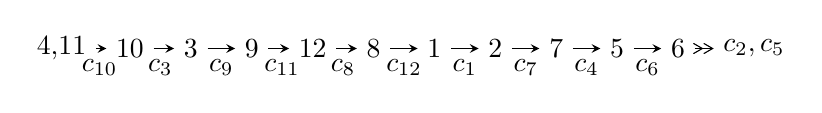
\begin{tikzpicture}[x=22pt, y=7pt]
	% node
	\node (A0) at (-1/8, 0) {4,11};
	\node (A1) at (1, 0) {10};
	\node (A2) at (2, 0) {3};
	\node (A3) at (3, 0) {9};
	\node (A4) at (4, 0) {12};
	\node (A5) at (5, 0) {8};
	\node (A6) at (6, 0) {1};
	\node (A7) at (7, 0) {2};
	\node (A8) at (8, 0) {7};
	\node (A9) at (9, 0) {5};
	\node (A10) at (10, 0) {6};
	\node (C1) at (1/2, -1) {$c_{10}$};
	\node (C2) at (3/2, -1) {$c_{3}$};
	\node (C3) at (5/2, -1) {$c_{9}$};
	\node (C4) at (7/2, -1) {$c_{11}$};
	\node (C5) at (9/2, -1) {$c_{8}$};
	\node (C6) at (11/2, -1) {$c_{12}$};
	\node (C7) at (13/2, -1) {$c_{1}$};
	\node (C8) at (15/2, -1) {$c_{7}$};
	\node (C9) at (17/2, -1) {$c_{4}$};
	\node (C10) at (19/2, -1) {$c_{6}$};
	\node (A11) at (45/4, 0) {$c_{2},c_{5}$};

	% edge
	\draw[->,>=stealth]	
	(A0) edge (A1) (A1) edge (A2) (A2) edge (A3) (A3) edge (A4) (A4) edge (A5) (A5) edge (A6) (A6) edge (A7) (A7) edge (A8) (A8) edge (A9) (A9) edge (A10) ;
	\draw[->>,>={angle 60}]	
	(A10) edge (A11);
\end{tikzpicture} \\ 

\end{tabular} \\

\footnotetext{
The image of knot diagram is generated by the software ``\textbf{Draw programme}" developed by Andrew Bartholomew(\url{http://www.layer8.co.uk/maths/draw/index.htm\#Running-draw}), where we modified some parts for our purpose(\url{https://github.com/CATsTAILs/LinksPainter}).
}\phantom \\ \newline 
\centering \textbf{Ideals for irreducible components\footnotemark of $X_{\text{par}}$} 
 
\begin{align*}
I^u_{1}&=\langle 
u^{40}+u^{39}+\cdots+2 u+1\rangle \\
\\
\end{align*}
\raggedright * 1 irreducible components of $\dim_{\mathbb{C}}=0$, with total 40 representations.\\
\footnotetext{All coefficients of polynomials are rational numbers. But the coefficients are sometimes approximated in decimal forms when there is not enough margin.}
\newpage
\renewcommand{\arraystretch}{1}
\centering \section*{I. $I^u_{1}= \langle u^{40}+u^{39}+\cdots+2 u+1 \rangle$}
\flushleft \textbf{(i) Arc colorings}\\
\begin{tabular}{m{7pt} m{180pt} m{7pt} m{180pt} }
\flushright $a_{4}=$&$\begin{pmatrix}0\\u\end{pmatrix}$ \\
\flushright $a_{11}=$&$\begin{pmatrix}1\\0\end{pmatrix}$ \\
\flushright $a_{10}=$&$\begin{pmatrix}1\\u^2\end{pmatrix}$ \\
\flushright $a_{3}=$&$\begin{pmatrix}- u\\- u^3+u\end{pmatrix}$ \\
\flushright $a_{9}=$&$\begin{pmatrix}- u^2+1\\u^2\end{pmatrix}$ \\
\flushright $a_{12}=$&$\begin{pmatrix}u^4- u^2+1\\- u^4\end{pmatrix}$ \\
\flushright $a_{8}=$&$\begin{pmatrix}- u^6+u^4-2 u^2+1\\u^6+u^2\end{pmatrix}$ \\
\flushright $a_{1}=$&$\begin{pmatrix}u^8- u^6+3 u^4-2 u^2+1\\- u^8-2 u^4\end{pmatrix}$ \\
\flushright $a_{2}=$&$\begin{pmatrix}u^{12}- u^{10}+5 u^8-4 u^6+6 u^4-3 u^2+1\\u^{14}-2 u^{12}+5 u^{10}-8 u^8+6 u^6-6 u^4+u^2\end{pmatrix}$ \\
\flushright $a_{7}=$&$\begin{pmatrix}- u^{10}+u^8-4 u^6+3 u^4-3 u^2+1\\u^{10}+3 u^6+u^2\end{pmatrix}$ \\
\flushright $a_{5}=$&$\begin{pmatrix}- u^{21}+2 u^{19}+\cdots+6 u^3- u\\u^{21}- u^{19}+7 u^{17}-6 u^{15}+16 u^{13}-11 u^{11}+13 u^9-6 u^7+3 u^5- u^3+u\end{pmatrix}$ \\
\flushright $a_{6}=$&$\begin{pmatrix}- u^{32}+3 u^{30}+\cdots-2 u^2+1\\u^{32}-2 u^{30}+\cdots-6 u^6+4 u^4\end{pmatrix}$\\&\end{tabular}
\flushleft \textbf{(ii) Obstruction class $= -1$}\\~\\
\flushleft \textbf{(iii) Cusp Shapes $= -4 u^{38}-4 u^{37}+12 u^{36}+16 u^{35}-68 u^{34}-76 u^{33}+160 u^{32}+212 u^{31}-468 u^{30}-552 u^{29}+872 u^{28}+1132 u^{27}-1696 u^{26}-2028 u^{25}+2496 u^{24}+3124 u^{23}-3500 u^{22}-4108 u^{21}+4004 u^{20}+4760 u^{19}-4124 u^{18}-4644 u^{17}+3528 u^{16}+3972 u^{15}-2596 u^{14}-2808 u^{13}+1496 u^{12}+1668 u^{11}-696 u^{10}-764 u^9+152 u^8+252 u^7+8 u^6-20 u^5-52 u^4-8 u^3+20 u^2+16 u-2$}\\~\\
\newpage\renewcommand{\arraystretch}{1}
\flushleft \textbf{(iv) u-Polynomials at the component}\newline \\
\begin{tabular}{m{50pt}|m{274pt}}
Crossings & \hspace{64pt}u-Polynomials at each crossing \\
\hline $$\begin{aligned}c_{1},c_{4},c_{6}\end{aligned}$$&$\begin{aligned}
&u^{40}+11 u^{39}+\cdots+4 u+1
\end{aligned}$\\
\hline $$\begin{aligned}c_{2},c_{5}\end{aligned}$$&$\begin{aligned}
&u^{40}+u^{39}+\cdots-2 u+1
\end{aligned}$\\
\hline $$\begin{aligned}c_{3},c_{10}\end{aligned}$$&$\begin{aligned}
&u^{40}+u^{39}+\cdots+2 u+1
\end{aligned}$\\
\hline $$\begin{aligned}c_{7},c_{8},c_{9}\\c_{11},c_{12}\end{aligned}$$&$\begin{aligned}
&u^{40}-7 u^{39}+\cdots-4 u+1
\end{aligned}$\\
\hline
\end{tabular}\\~\\
\newpage\renewcommand{\arraystretch}{1}
\flushleft \textbf{(v) Riley Polynomials at the component}\newline \\
\begin{tabular}{m{50pt}|m{274pt}}
Crossings & \hspace{64pt}Riley Polynomials at each crossing \\
\hline $$\begin{aligned}c_{1},c_{4},c_{6}\end{aligned}$$&$\begin{aligned}
&y^{40}+37 y^{39}+\cdots+12 y+1
\end{aligned}$\\
\hline $$\begin{aligned}c_{2},c_{5}\end{aligned}$$&$\begin{aligned}
&y^{40}-11 y^{39}+\cdots-4 y+1
\end{aligned}$\\
\hline $$\begin{aligned}c_{3},c_{10}\end{aligned}$$&$\begin{aligned}
&y^{40}-7 y^{39}+\cdots-4 y+1
\end{aligned}$\\
\hline $$\begin{aligned}c_{7},c_{8},c_{9}\\c_{11},c_{12}\end{aligned}$$&$\begin{aligned}
&y^{40}+53 y^{39}+\cdots+20 y+1
\end{aligned}$\\
\hline
\end{tabular}\\~\\
\newpage\flushleft \textbf{(vi) Complex Volumes and Cusp Shapes}
$$\begin{array}{c|c|c}  
\text{Solutions to }I^u_{1}& \I (\text{vol} + \sqrt{-1}CS) & \text{Cusp shape}\\
 \hline 
\begin{aligned}
u &= -0.774023 + 0.626573 I\end{aligned}
 & -2.27514 - 2.35684 I & \phantom{-}1.32722 + 3.76894 I \\ \hline\begin{aligned}
u &= -0.774023 - 0.626573 I\end{aligned}
 & -2.27514 + 2.35684 I & \phantom{-}1.32722 - 3.76894 I \\ \hline\begin{aligned}
u &= \phantom{-}0.739124 + 0.708073 I\end{aligned}
 & -5.26679 - 0.18413 I & -6.20607 + 0.92237 I \\ \hline\begin{aligned}
u &= \phantom{-}0.739124 - 0.708073 I\end{aligned}
 & -5.26679 + 0.18413 I & -6.20607 - 0.92237 I \\ \hline\begin{aligned}
u &= \phantom{-}0.627832 + 0.730855 I\end{aligned}
 & \phantom{-}0.73402 - 4.48374 I & -0.96535 + 2.86050 I \\ \hline\begin{aligned}
u &= \phantom{-}0.627832 - 0.730855 I\end{aligned}
 & \phantom{-}0.73402 + 4.48374 I & -0.96535 - 2.86050 I \\ \hline\begin{aligned}
u &= -0.608675 + 0.698819 I\end{aligned}
 & \phantom{-}1.19980 - 1.38740 I & -0.07893 + 2.54985 I \\ \hline\begin{aligned}
u &= -0.608675 - 0.698819 I\end{aligned}
 & \phantom{-}1.19980 + 1.38740 I & -0.07893 - 2.54985 I \\ \hline\begin{aligned}
u &= \phantom{-}0.838818 + 0.669942 I\end{aligned}
 & -4.94096 + 5.29818 I & -4.71903 - 7.91162 I \\ \hline\begin{aligned}
u &= \phantom{-}0.838818 - 0.669942 I\end{aligned}
 & -4.94096 - 5.29818 I & -4.71903 + 7.91162 I \\ \hline\begin{aligned}
u &= -0.898655 + 0.598871 I\end{aligned}
 & \phantom{-}2.12810 - 3.44087 I & \phantom{-}2.44727 + 3.96002 I \\ \hline\begin{aligned}
u &= -0.898655 - 0.598871 I\end{aligned}
 & \phantom{-}2.12810 + 3.44087 I & \phantom{-}2.44727 - 3.96002 I \\ \hline\begin{aligned}
u &= -0.891111 + 0.219846 I\end{aligned}
 & \phantom{-}6.32393 - 5.42631 I & \phantom{-}7.65967 + 7.06500 I \\ \hline\begin{aligned}
u &= -0.891111 - 0.219846 I\end{aligned}
 & \phantom{-}6.32393 + 5.42631 I & \phantom{-}7.65967 - 7.06500 I \\ \hline\begin{aligned}
u &= \phantom{-}0.888297 + 0.191636 I\end{aligned}
 & \phantom{-}6.47477 - 0.62864 I & \phantom{-}8.33631 - 1.45489 I \\ \hline\begin{aligned}
u &= \phantom{-}0.888297 - 0.191636 I\end{aligned}
 & \phantom{-}6.47477 + 0.62864 I & \phantom{-}8.33631 + 1.45489 I \\ \hline\begin{aligned}
u &= \phantom{-}0.908694 + 0.617877 I\end{aligned}
 & \phantom{-}1.65204 + 9.48216 I & \phantom{-}1.43346 - 8.89660 I \\ \hline\begin{aligned}
u &= \phantom{-}0.908694 - 0.617877 I\end{aligned}
 & \phantom{-}1.65204 - 9.48216 I & \phantom{-}1.43346 + 8.89660 I \\ \hline\begin{aligned}
u &= -0.738242 + 0.308879 I\end{aligned}
 & \phantom{-}0.00908 - 2.86239 I & \phantom{-}2.01297 + 9.95605 I \\ \hline\begin{aligned}
u &= -0.738242 - 0.308879 I\end{aligned}
 & \phantom{-}0.00908 + 2.86239 I & \phantom{-}2.01297 - 9.95605 I \\ \hline\begin{aligned}
u &= \phantom{-}0.914966 + 0.925195 I\end{aligned}
 & -7.90110 + 0.93902 I & \phantom{-0.000000 } 0. - 2.11894 I \\ \hline\begin{aligned}
u &= \phantom{-}0.914966 - 0.925195 I\end{aligned}
 & -7.90110 - 0.93902 I & \phantom{-0.000000 -}0. + 2.11894 I \\ \hline\begin{aligned}
u &= \phantom{-}0.687807 + 0.092383 I\end{aligned}
 & \phantom{-}1.071350 + 0.173422 I & \phantom{-}9.40169 - 0.46654 I \\ \hline\begin{aligned}
u &= \phantom{-}0.687807 - 0.092383 I\end{aligned}
 & \phantom{-}1.071350 - 0.173422 I & \phantom{-}9.40169 + 0.46654 I \\ \hline\begin{aligned}
u &= -0.915560 + 0.932311 I\end{aligned}
 & -8.66424 + 5.12373 I & -1.21591 - 2.77049 I \\ \hline\begin{aligned}
u &= -0.915560 - 0.932311 I\end{aligned}
 & -8.66424 - 5.12373 I & -1.21591 + 2.77049 I \\ \hline\begin{aligned}
u &= \phantom{-}0.940784 + 0.913719 I\end{aligned}
 & -11.90030 + 3.36395 I & \phantom{-0.000000 } 0. - 2.30636 I \\ \hline\begin{aligned}
u &= \phantom{-}0.940784 - 0.913719 I\end{aligned}
 & -11.90030 - 3.36395 I & \phantom{-0.000000 -}0. + 2.30636 I \\ \hline\begin{aligned}
u &= \phantom{-}0.963476 + 0.899832 I\end{aligned}
 & -7.74288 + 5.77907 I & \phantom{-0.000000 } 0. - 2.48353 I \\ \hline\begin{aligned}
u &= \phantom{-}0.963476 - 0.899832 I\end{aligned}
 & -7.74288 - 5.77907 I & \phantom{-0.000000 -}0. + 2.48353 I\\
 \hline 
 \end{array}$$\newpage$$\begin{array}{c|c|c}  
\text{Solutions to }I^u_{1}& \I (\text{vol} + \sqrt{-1}CS) & \text{Cusp shape}\\
 \hline 
\begin{aligned}
u &= -0.936757 + 0.927705 I\end{aligned}
 & -15.3144 - 0.1076 I & -5.83673 - 1.11315 I \\ \hline\begin{aligned}
u &= -0.936757 - 0.927705 I\end{aligned}
 & -15.3144 + 0.1076 I & -5.83673 + 1.11315 I \\ \hline\begin{aligned}
u &= -0.954303 + 0.917987 I\end{aligned}
 & -15.2565 - 6.6798 I & -5.66567 + 5.71643 I \\ \hline\begin{aligned}
u &= -0.954303 - 0.917987 I\end{aligned}
 & -15.2565 + 6.6798 I & -5.66567 - 5.71643 I \\ \hline\begin{aligned}
u &= -0.968399 + 0.903607 I\end{aligned}
 & -8.4907 - 11.8771 I & -0.89615 + 7.29232 I \\ \hline\begin{aligned}
u &= -0.968399 - 0.903607 I\end{aligned}
 & -8.4907 + 11.8771 I & -0.89615 - 7.29232 I \\ \hline\begin{aligned}
u &= -0.027916 + 0.568771 I\end{aligned}
 & \phantom{-}3.61497 + 2.92206 I & -0.55528 - 2.79244 I \\ \hline\begin{aligned}
u &= -0.027916 - 0.568771 I\end{aligned}
 & \phantom{-}3.61497 - 2.92206 I & -0.55528 + 2.79244 I \\ \hline\begin{aligned}
u &= -0.296155 + 0.379057 I\end{aligned}
 & -1.252400 + 0.309569 I & -6.95116 - 0.49193 I \\ \hline\begin{aligned}
u &= -0.296155 - 0.379057 I\end{aligned}
 & -1.252400 - 0.309569 I & -6.95116 + 0.49193 I\\
 \hline 
 \end{array}$$\newpage
\newpage\renewcommand{\arraystretch}{1}
\centering \section*{ II. u-Polynomials}
\begin{tabular}{m{50pt}|m{274pt}}
Crossings & \hspace{64pt}u-Polynomials at each crossing \\
\hline $$\begin{aligned}c_{1},c_{4},c_{6}\end{aligned}$$&$\begin{aligned}
&u^{40}+11 u^{39}+\cdots+4 u+1
\end{aligned}$\\
\hline $$\begin{aligned}c_{2},c_{5}\end{aligned}$$&$\begin{aligned}
&u^{40}+u^{39}+\cdots-2 u+1
\end{aligned}$\\
\hline $$\begin{aligned}c_{3},c_{10}\end{aligned}$$&$\begin{aligned}
&u^{40}+u^{39}+\cdots+2 u+1
\end{aligned}$\\
\hline $$\begin{aligned}c_{7},c_{8},c_{9}\\c_{11},c_{12}\end{aligned}$$&$\begin{aligned}
&u^{40}-7 u^{39}+\cdots-4 u+1
\end{aligned}$\\
\hline
\end{tabular}\newpage\renewcommand{\arraystretch}{1}
\centering \section*{ III. Riley Polynomials}
\begin{tabular}{m{50pt}|m{274pt}}
Crossings & \hspace{64pt}Riley Polynomials at each crossing \\
\hline $$\begin{aligned}c_{1},c_{4},c_{6}\end{aligned}$$&$\begin{aligned}
&y^{40}+37 y^{39}+\cdots+12 y+1
\end{aligned}$\\
\hline $$\begin{aligned}c_{2},c_{5}\end{aligned}$$&$\begin{aligned}
&y^{40}-11 y^{39}+\cdots-4 y+1
\end{aligned}$\\
\hline $$\begin{aligned}c_{3},c_{10}\end{aligned}$$&$\begin{aligned}
&y^{40}-7 y^{39}+\cdots-4 y+1
\end{aligned}$\\
\hline $$\begin{aligned}c_{7},c_{8},c_{9}\\c_{11},c_{12}\end{aligned}$$&$\begin{aligned}
&y^{40}+53 y^{39}+\cdots+20 y+1
\end{aligned}$\\
\hline
\end{tabular}
\vskip 2pc
\end{document}